\documentclass[tikz]{standalone}
\usepackage{tikz}
\usepackage{graphicx}

\usetikzlibrary{calc, angles, quotes}
\usetikzlibrary{intersections} % Necessário para achar pontos de cruzamento

\begin{document}
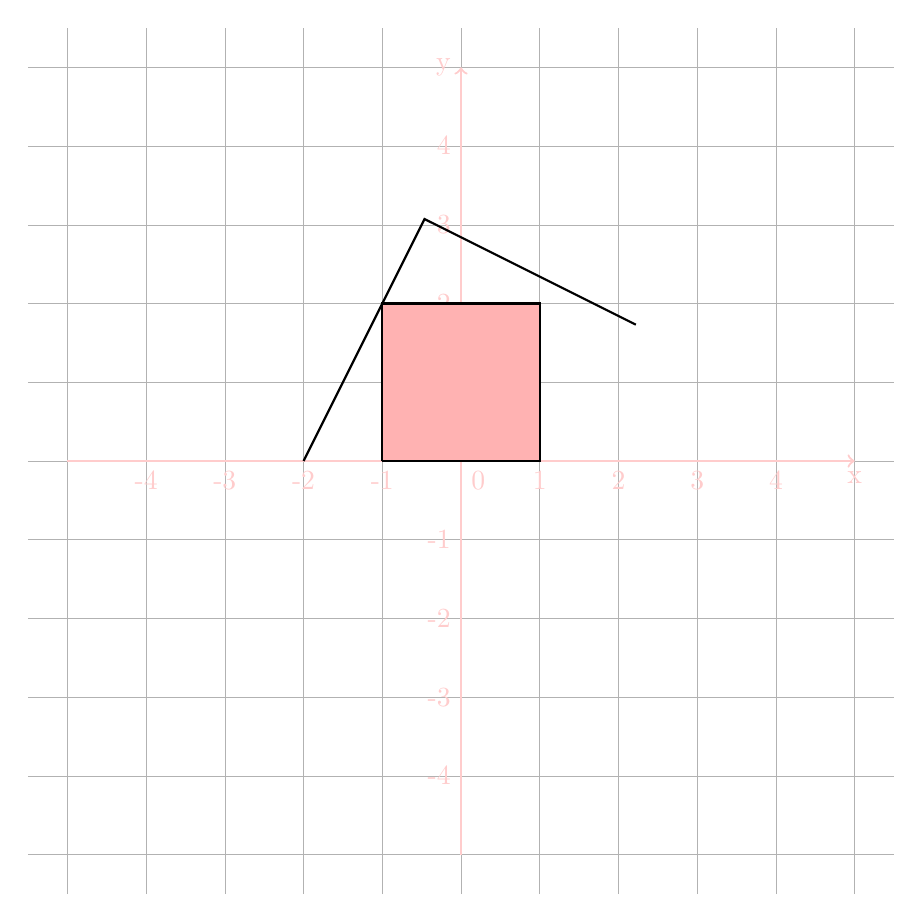
\begin{tikzpicture}[thick]

  \draw[help lines,black!30] (-5.5,-5.5) grid (5.5,5.5);
  \draw[thick,->,red!20] (0,-5) -- (0,5) node[left]  {y};
  \draw[thick,->,red!20] (-5,0) -- (5,0) node[below] {x};
  \foreach \x in {-4,-3,-2,-1,1,2,3,4} \node[left,color=red!20] at (0,\x) {\x} node[below,color=red!20] at (\x,0) {\x};
  \node[below right,color=red!20] at (0,0) {0}; 
   

  \draw[fill=red!30] (-1,0) coordinate (a) -- 
        (-1,2) coordinate (b) -- 
        (1,2)  coordinate (c) -- 
        (1,0)  coordinate (d) -- 
        (-1,0);
  
  \draw (-2,0) coordinate (A) -- ($(b)!-1.2cm!(A)$) coordinate (B) -- ($(B)!3cm!90:(A)$);

  %\node[left]  at ($(a)!.5!(b)$) {$x$};
  %\node[above] at ($(c)!.5!(b)$) {$x$};
  %\node[right] at ($(c)!.5!(d)$) {$x$};
  %\node[below] at ($(a)!.5!(d)$) {$x$};
%
  %\draw (-2,0) coordinate (A) -- ($(b)!-1.2cm!(A)$) coordinate (B);
  %\path[name path=line1]  (B) -- ($(c)!-4cm!(B)$);
  %\path[name path=line2,thick,red] (A) -- (4,0);
%
  %\fill[red, name intersections={of=line1 and line2, by=C}] (C);
  %\draw (A) -- (C);
  %\draw (B) -- (C);
 
\end{tikzpicture}


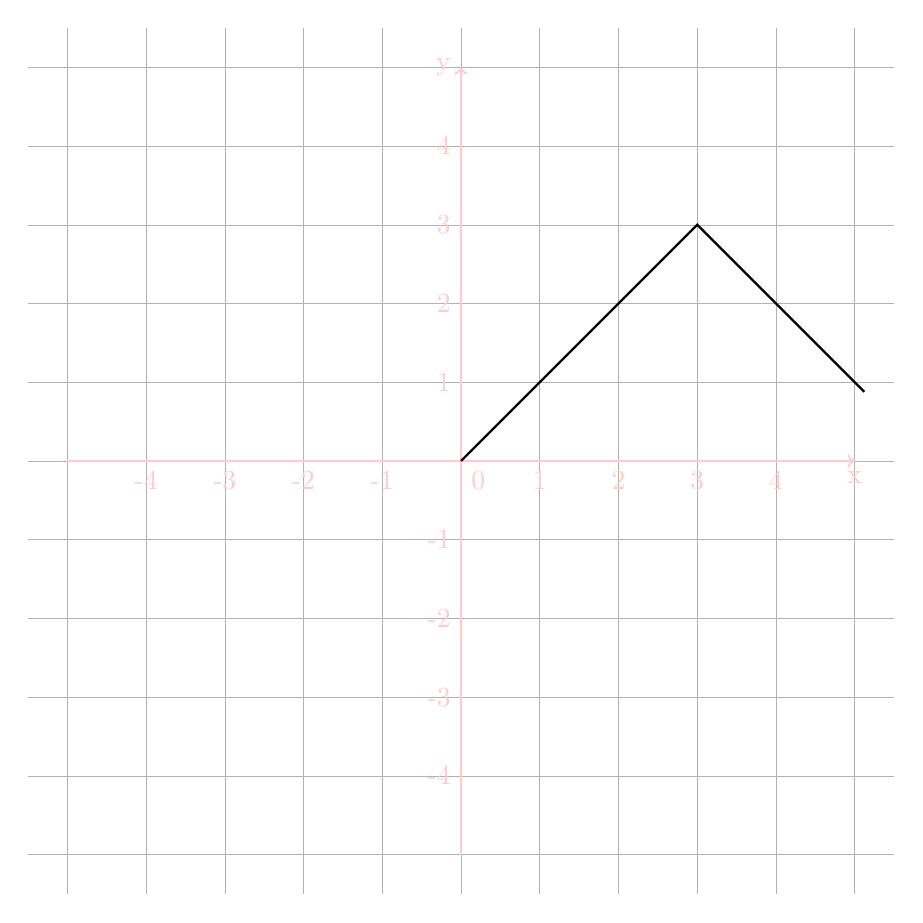
\begin{tikzpicture}[thick]

  \draw[help lines,black!30] (-5.5,-5.5) grid (5.5,5.5);
  \draw[thick,->,red!20] (0,-5) -- (0,5) node[left]  {y};
  \draw[thick,->,red!20] (-5,0) -- (5,0) node[below] {x};
  \foreach \x in {-4,-3,-2,-1,1,2,3,4} \node[left,color=red!20] at (0,\x) {\x} node[below,color=red!20] at (\x,0) {\x};
  \node[below right,color=red!20] at (0,0) {0}; 
   

\draw (0,0) coordinate (A) -- (3,3) coordinate (B) -- ($(B)!3cm!90:(A)$) ;

\end{tikzpicture}


\end{document}